\documentclass[11pt]{article}

\usepackage{"../../info/packages"}
\usepackage{"../../info/nomenclature"}
\usepackage{fullpage}


\title{Functional analysis}
\author{Alejandro Campos}

\begin{document}

\maketitle
\tableofcontents

%--------------------------------------------------------------------------
\section{Linear forms}
%--------------------------------------------------------------------------
\begin{itemize}

    \item A linear form (or linear functional) is a mapping $w:V \to \mathbb{R}$ such that
    \begin{equation}
        w(\vvec_1 + \vvec_2) = w(\vvec_1) + w(\vvec_2) \qquad \forall \vvec_1, \vvec_2 \in V,
    \end{equation}
    \begin{equation}
        w(\alpha \vvec) = \alpha w(\vvec) \qquad \forall \alpha \in \mathbb{R}, \vvec \in V.
    \end{equation}

    \item A bilinear form (or bilinear functional) is a mapping $w: V \times U \to \mathbb{R}$ such that
    \begin{equation}
        w(\vvec_1 + \vvec_2, \uvec) = w(\vvec_1, \uvec) + w(\vvec_2, \uvec) \qquad \forall \vvec_1, \vvec_2 \in V, \uvec \in U, 
    \end{equation}
    \begin{equation}
        w(\vvec, \uvec_1 + \uvec_2) = w(\vvec, \uvec_1) + w(\vvec, \uvec_2) \qquad \forall \vvec \in V, \uvec_1, \uvec_2 \in U, 
    \end{equation}
    \begin{equation}
        w(\alpha \vvec, \uvec) = \alpha w(\vvec, \uvec) \qquad \forall \alpha \in \mathbb{R}, \vvec \in V, \uvec \in U,
    \end{equation}
    \begin{equation}
        w(\vvec, \alpha \uvec) = \alpha w(\vvec, \uvec) \qquad \forall \alpha \in \mathbb{R}, \vvec \in V, \uvec \in U,
    \end{equation}

    \item A multi-linear form (or multi-linear functional) is a mapping $w: V^{(1)} \times ... V^{(n)} \to \mathbb{R}$ such that
    \begin{equation}
        w(\vvec^{(1)}, ..., \vvec^{(i)}_1 + \vvec^{(i)}_2, ... , \vvec^{(n)}) = w(\vvec^{(1)}, ..., \vvec^{(i)}_1, ... , \vvec^{(n)}) + w(\vvec^{(1)}, ..., \vvec^{(i)}_2, ... , \vvec^{(n)}),
    \end{equation}
    \begin{equation}
        w(\vvec^{(1)}, ..., \alpha \vvec^{(i)}, ... , \vvec^{(n)}) = \alpha w(\vvec^{(1)}, ..., \vvec^{(i)}, ... , \vvec^{(n)}),
    \end{equation}
    $\forall i$, $\forall \alpha \in \mathbb{R}$, $\forall \vvec^{(1)} \in V^{(1)}$, ... , $\forall \vvec^{(n)} \in V^{(n)}$, and $\forall \vvec^{(i)}_1, \vvec^{(i)}_2 \in V^{(i)}$.

\end{itemize}

%---------------------------------------------------------------
\section{Some terminology}
%---------------------------------------------------------------
\begin{itemize}
    \item Cauchy sequence: a sequence $v_1$, $v_2$, $v_3$, ... \@is a Cauchy sequence if for every possitive real number $\epsilon$, there is a possitive integer $N$ such that for all possitive integers $m,n>N$, $||v_m-v_n||<\epsilon$. 
    \item Complete inner produce space: an inner product space $\mathcal{V}$ is complete if every Cauchy sequence $\{v_i\}_{i=1}^\infty$ in $\mathcal{V}$ has a limit $v = \lim v_i \in \mathcal{V}$.
    \item Compact set: a set is compact if it is bounded and closed.
    \item Coercive bilinear form: a bilinear form $a(:,:)$ is coercive in a Hilbert space $\mathcal{V}$ if 
    \begin{equation}
        a(v,v) \ge \alpha ||v||_\mathcal{V}^2, \qquad \forall v \in \mathcal{V}, \qquad \text{with }\alpha > 0.
    \end{equation}
    \item Bounded linear form: a linear form is bounded in the normed vector space $\mathcal{V}$ if there exists an $M>0$ such that $|L(v)| \le M ||v||$, for every $v \in \mathcal{V}$. 
    \item Bounded bilinear form: a bilinear form is bounded in the normed vector space $\mathcal{V}$ if there exists and $M>0$ such that $|a(w,v)| \le M ||w||\;||v||$, for every $w,v \in \mathcal{V}$.
\end{itemize}

%---------------------------------------------------------------
\section{Useful equalities and inequalities}
%---------------------------------------------------------------
\begin{align}
    &|ab| = |a||b| \qquad \forall a,b \in \mathbb{C} \\
    &|a + b| \le |a| + |b| \qquad \forall a,b \in \mathbb{C} \\
    &|(w,v)| \le ||w||\;||v|| \qquad \forall v,w \in \text{Inner product space (Cauchy-Schwarz inequality)} \\
    &||w + v|| \le ||w|| + ||v|| \qquad \forall v,w \in \text{Normed space (triangle inequality)} \\
    &\left | \int_a^b v(x) \, dx \right| \le \int_a^b |v(x)| \, dx \\
    &\left \| \int_a^b v(x,y) \, dx \right \| \le \int_a^b ||v(x,y)|| \, dx \text{ where the norm is over the y-domain}.
\end{align}

%---------------------------------------------------------------
\section{The weak derivative}
%---------------------------------------------------------------
If $v \in C^1(\bar{\Omega})$, then through integration by parts
\begin{equation}
    \int_\Omega \frac{\partial v}{\partial x_i} \phi \, dV = -\int_\Omega v \frac{\partial \phi}{\partial x_i} \, dV \qquad \forall \phi \in C_0^1(\Omega).
\end{equation}
However, if $v \in L_2(\Omega)$ but not necessarily in $C^1(\bar{\Omega})$, we cannot write the equation above. Instead, we ask, is there a function $w$ such that the following holds?
\begin{equation}
     \int_\Omega w \phi \, dV = -\int_\Omega v \frac{\partial \phi}{\partial x_i} \, dV \qquad \forall \phi \in C_0^1(\Omega).
\end{equation}
This can be rewritten as $(w,\phi) = L(\phi)$, where $L(\phi) = -\int_\Omega v \frac{\partial \phi}{\partial x_i} dV$. If $L(\phi)$ is bounded in $L_2$, Riesz' representation theorem then states a unique solution $w \in L_2(\Omega)$ exists. This $w$ is the weak derivative.

More generally, if $v \in C^k(\bar{\Omega})$, then through integration by parts
\begin{equation}
    \int_\Omega D^\alpha v \phi \, dV = (-1)^{|\alpha|} \int_\Omega v D^\alpha \phi \, dV \qquad \forall |\alpha| \le k,\, \forall \phi \in C_0^{|\alpha|}(\Omega).
\end{equation}
However, if $v \in L_2(\Omega)$ but not necessarily in $C^k(\bar{\Omega})$, we cannot write the equation above. Instead, we ask, is there a function $w$ such that the following holds?
\begin{equation}
    \int_\Omega w \phi \, dV = (-1)^{|\alpha|} \int_\Omega v D^\alpha \phi \, dV \qquad \forall \phi \in C_0^{|\alpha|}(\Omega).
\end{equation}
As before, if the left-hand-side operator is bounded, then we have a unique solution $w \in L_2(\Omega)$. This $w$ is the weak derivative. Often, weak derivatives are referred to as ``$D^\alpha v$ in the weak sense.''

%---------------------------------------------------------------
\section{Function spaces}
%---------------------------------------------------------------
We label function spaces using \textbackslash mathcal notation, except for the three main function spaces for continuous, square-integrable, and Sobolev functions. 
\begin{itemize}
    \item $C^0$: the set of all continuous functions
    \item $C^k$ the set of all functions whose derivatives up to order $k$ all exist and are continuous. These are called continuously differentiable functions of order $k$.
    \item $L_2$: the set of all functions that are square integrable.
    \item $H^k$: the set of all $L_2$ functions whose weak partial derivatives up to order $k$ also belong to $L_2$. 
    \item Let $\Omega$ be a bounded domain in $\mathbb{R}^d$ with smooth or polygonal boundary. Then part of the Sobolev embedding theorem can be written as
    \begin{equation}
        H^k(\Omega) \subset C^l(\bar{\Omega}) \text{ if } k > l + d/2.
    \end{equation}
    Thus, we have $H^m(\Omega) \subset C^{m-1}(\bar{\Omega})$ for $\Omega \in \mathbb{R}$ and $H^m(\Omega) \subset C^{m-2}(\bar{\Omega})$ for $\Omega \in \mathbb{R}^2$ or $\mathbb{R}^3$.
\end{itemize}

\begin{figure}[ht]
   \centering
   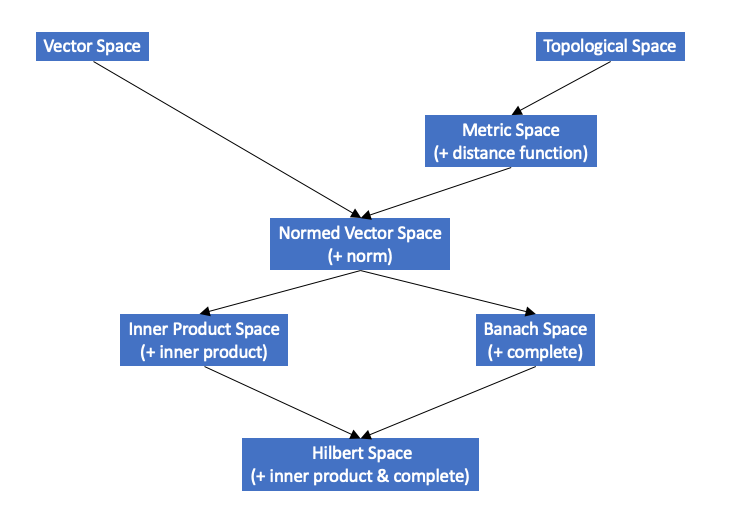
\includegraphics[width=0.8\textwidth]{../../images/function_spaces.png}
   \caption{Map of function spaces.}
   \label{fig:function_spaces}
\end{figure}

\setlength{\cellspacetoplimit}{3pt}
\setlength{\cellspacebottomlimit}{3pt}

\begin{center}
\begin{tabular}{Sc|Sc|Sc}
    Space & Norm & Inner product \\
    \hline
    $C(M)$ & $ \displaystyle ||v||_C = \sup_{x \in M} |v(x)| $ & X \\
    \hline
    $C^k(M)$ & $\begin{aligned} &||v||_{C^k} = \max_{|\alpha| \le k} ||D^\alpha v||_C \\ &|v|_{C^k}=\max_{|\alpha| = k} ||D^\alpha v||_C \end{aligned}$ & X \\
    \hline
    $L_p(\Omega)$ & $ \displaystyle ||v||_{L_p} = \left ( \int_\Omega |v|^p \, dV \right)^{1/p} $ & X \\
    \hline
    $L_2(\Omega)$ & $ \displaystyle ||v||_{L_2} = \left ( \int_\Omega |v|^2 \, dV \right)^{1/2} $ & $ \displaystyle (v,w) = \int_\Omega vw^* \, dV $ \\
    \hline
    $H^k(\Omega)$ & $ \begin{aligned} &||v||_k = \left ( \sum_{|\alpha| \le k} ||D^\alpha v||^2 \right )^{1/2} \\ &|v|_k = \left ( \sum_{|\alpha| = k} ||D^\alpha v||^2 \right )^{1/2} \end{aligned}$ & $ \displaystyle (v,w)_k = \sum_{|\alpha \le k|} (D^\alpha v, D^\alpha w) $
\end{tabular}
\end{center}

\end{document}